\subsubsection{$H \to \gamma\gamma$}
\label{sec:Hgammagamma}
%% {\it To be written by: M. Delmastro}

\newcommand{\Hyy}{\hbox{$H\to\gamma\gamma$}}

The measurement of the Higgs boson properties in the \Hyy\ is extrapolated from the most recent measurements by ATLAS with 80\,$\mathrm{fb}^{-1}$ \cite{ATLAS:2018uso} and CMS with XX\,$\mathrm{fb}^{-1}$ \cite{}.

Events are selected to contain two isolated photon candidates passing good quality requirements in the precision regions of the detectors. Events are further segmented according to the objects campaigning the diphoton system, in order to maximize the sensitivity to the main Higgs production modes ($ggH+b\bar{b}H$, VBF, $VH$ = $qqZH+ggZH+WH$ and top = $t\bar{t}H+tH$) and to reduce the uncertainties on the respective cross sections, as well as to the Simplified Template Cross Section (STXS, first introduced in Refs \cite{}) in the merged version of Stage-1. These cross sections are measured for a Higgs boson absolute rapidity $|y_H|$ smaller than 2.5, and with further requirements on the associated objects (e.g. jet $p_\mathrm{T}$).

The \Hyy\ signal is extracted by means of a combined signal-plus-background fit, where both the continuous background and the signal resonance are parameterized by analytical functions. The shape properties of the signal PDF are obtained by MC simulation, and constrained by performance studies of the photon energy scale and resolution. The background PDF is completely determined by the fit on data, with systematic uncertainties attributed to the specific choice of functional form \cite{} or using a profiling method \cite{}.

The main systematic uncertainties affecting the results are the background modelling uncertainty, QCD scale uncertainties causing event migrations between the bins, photon isolation efficiencies and jet uncertainties.
%% Beside that, the underlying event and parton showering uncertainties as well as the PES and PER play are role.
%
On top of the common assumptions mentioned in Section~\ref{sec:HiggsExtrapAss}, the ATLAS \Hyy\ results include a 10\% increase of the background modeling systematic uncertainties, to account for the potentially worst knowledge of the background composition in each analysis category at HL-LHC: this assumption has anyway negligible impact.
%
In the Run-2 analyses, a conservative 100\% uncertainty on the heavy flavour resonant background in top-sensitive categories is applied. Measurements by ATLAS and CMS of the heavy flavour content, or the $b$-jet multiplicity, are expected to better constrain these contributions: for the S2 scenario extrapolation, this uncertainty is therefore halved.

Figure~\ref{fig:Hyy_ATLAS_HLLHC_S2} show the ratio of the extrapolated ATLAS measurements of the main four Higgs production modes to their respective theoretical SM predictions. The reduction of the total uncertainty with respect to the 80\,$\mathrm{fb}^{-1}$ results ranges from a factor 2(3) for the S1 (S2) scenario for the $ggH+b\bar{b}H$, VBF, top cross sections, to a factor 5(6) for the $VH$ cross section.

\begin{figure}
  \centering
  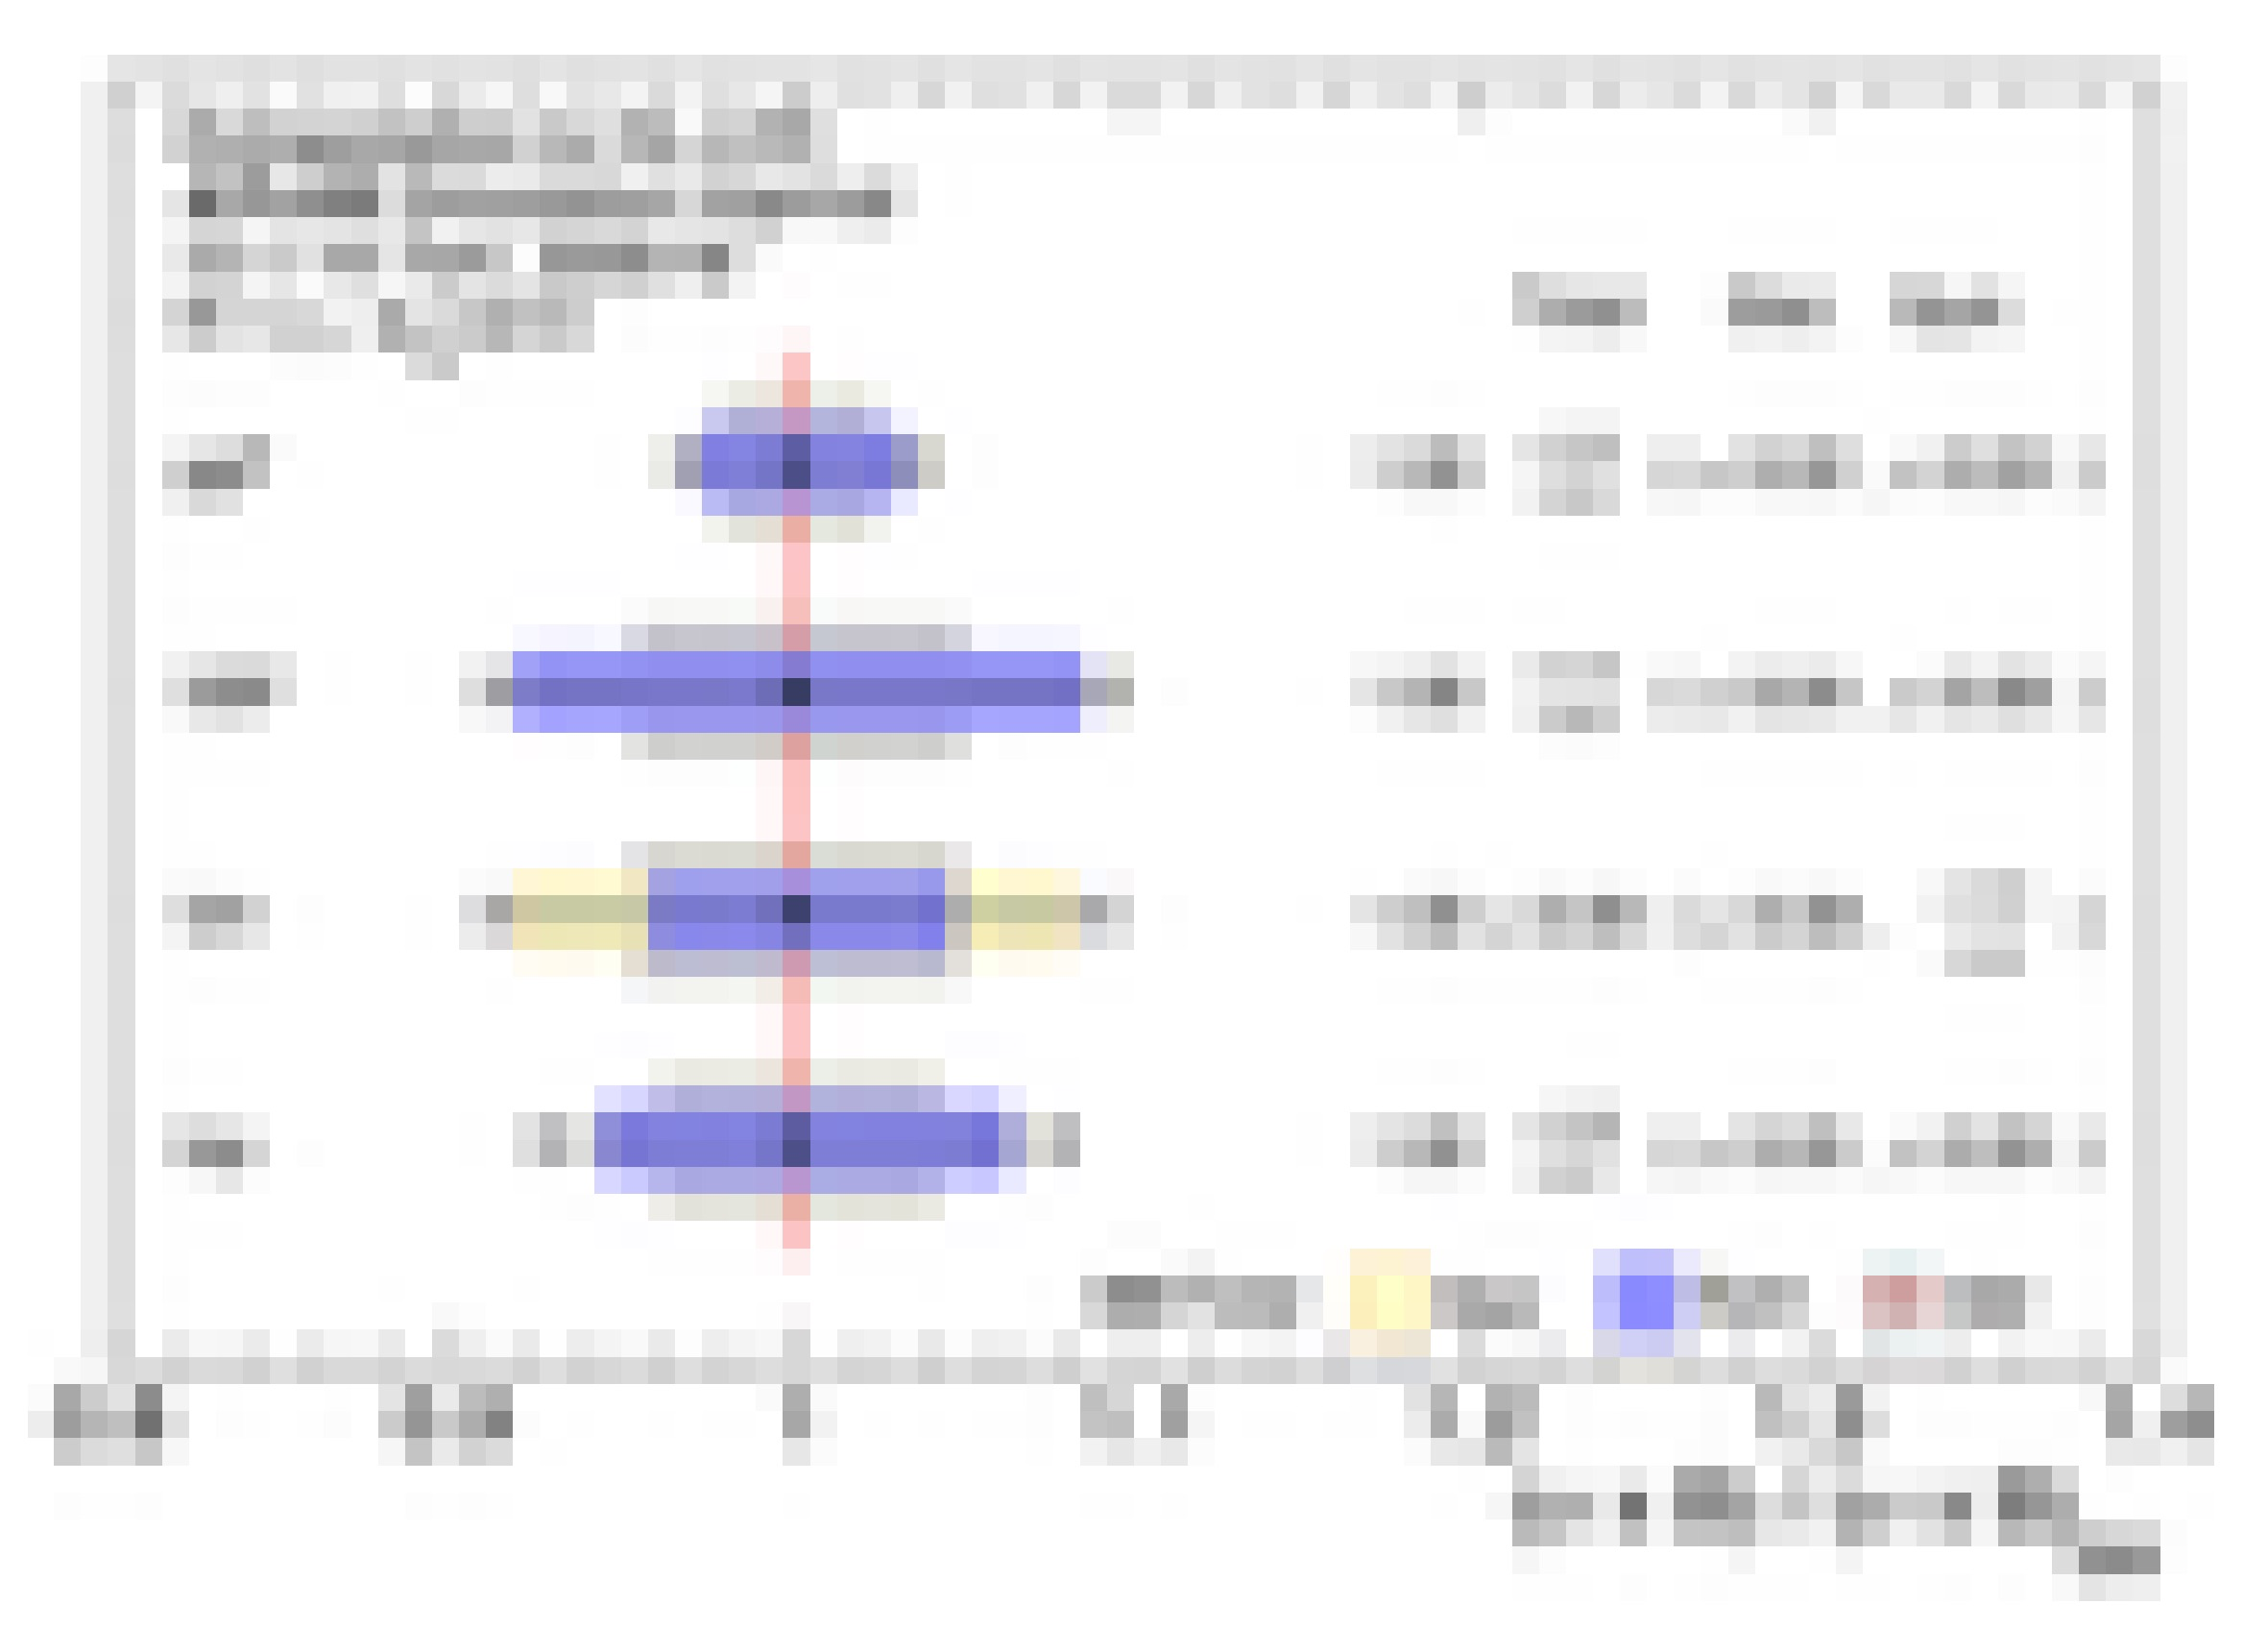
\includegraphics[width=0.6\linewidth]{section2/plots/channels/ATLAS_Hyy_compareToSM_prodXS}
  \caption{Ratio of the measurements of the main four Higgs production modes in the \Hyy\ decay channel to their respective theoretical SM predictions, as extrapolated at the HL-LHC for scenario S2 by ATLAS.}
  \label{fig:Hyy_ATLAS_HLLHC_S2}
\end{figure}


\subsubsection{$H \to Z\gamma \to 2\ell\,\gamma$}
{\it To be written by: M. Delmastro}

\subsubsection{$H \to ZZ^* \to 4\ell$}
{\it To be written by: M. Delmastro}

\subsubsection{$H \to WW^* \to \ell\nu\,\ell\nu$}
{\it To be written by: M. Delmastro}